\mySection{10.1 Introduction}
%-------------- start slide -------------------------------%{{{ 10.4
\begin{frame}
	\centering
	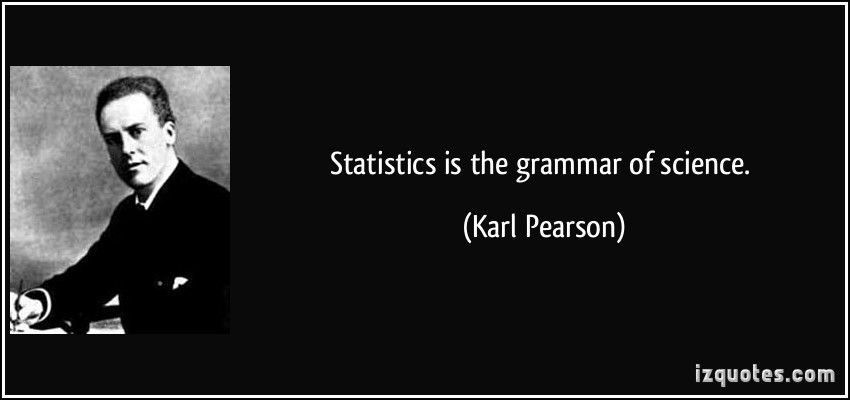
\includegraphics[scale=0.4]{Pearson_quote.jpg}
	\vfill
	\begin{enumerate}
		\item Karl Pearson, 1857 -- 1936.
		\item English mathematician and biostatistician.
		\item He has been credited with establishing the discipline of mathematical statistics
		\item Method of moments; p-Value; \underline{Chi-square test}; Foundations of statistical hypothesis testing theory; principle component analysis ...
	\end{enumerate}
\end{frame}
%-------------- end slide -------------------------------%}}}
%-------------- start slide -------------------------------%{{{ 10.5
\begin{frame}
\centering
Pearson's chi-squared test\\ in one shot
\vfill

\includegraphics[scale=0.15]{Goodness_fit_test_puzzle-neg.png}
\vfill
\[
	\chi^2 =\sum  \frac{ \left( \text{Observed} - \text{Expected} \right)^2 }{\text{Expected}} \sim \text{Chi Square of $df$}
\]
\vfill
\[
	df = \text{numer of classes} -\text{number of estimated parameters} - 1
\]
\vfill
All expected $\ge 5$
\end{frame}
%-------------- end slide -------------------------------%}}}
